During August 2022 a testbeam took place in Santa Chiara hospital in Pisa, where a new accelerator designed for both medical research and R$\&$D on FLASH-RT, and for this reason called "ElectronFlash", have been installed a few months ago. 
The motivation of the testbeam measurements were testing TJ-Mopopix1 at high dose rate with a focus on investigating the possibility of the application in radiotherapy. Despite this particular device does not seem fitting the requirements imposed for that application, especially regarding the readout time, the measurements have been useful since help us charaterizing the setup for future advance, and also give us the possibility of a complete charaterization of the chip.
\begin{figure}
   \centering
   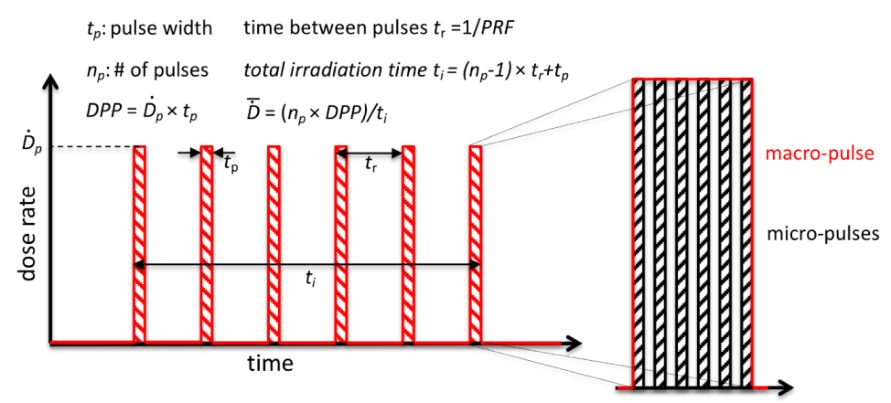
\includegraphics[width=.9\linewidth]{figures/test_beam/beam_structure.pdf}
   \caption{Typical beam structure of a beam used in electron radiotherapy}
   \label{fig:beam_structure}
\end{figure}

Given that in medical physics the dose is the standard parameter to charaterize the beam, beacause of its obvious relation with the damage caused in the patient, I am going to explain the meaning of it by the point of view of the instrumentation.
Infact, when interacting with measuring systems a more common and usefull parameter is the rate or the fluence of particles.
The conversion between the two quantity can be find thinking to the definition of dose: it is the concentration of energy deposited in tissue as a result of an exposure to ionizing radiation. 
Assuming total absorption of electrons in water, defined by law as the ordinarily reference medium, the dose can be expressed as: 
\begin{equation}
   D[Gy] = \frac{N E[eV]}{\rho[g/cm^3] A[cm^2] x[cm]}
\end{equation}
After having applyed the conversion of the energy from \si{eV} to \si{J} and noticed that E/$\rho$x roughly corresponds to the stopping power S of electrons in water, a simple estimation of the dose released in water is:
\begin{equation}
   D[Gy] = 1.602\;10^{-10}\,N[cm^{-2}]\,S[MeV cm^2/g]
\end{equation}

\section{Apparatus description}
   In order to shield the outdoor from ionizing radiation the accelerator is placed in a bunker inside the hospital. The bunker has very thick walls of cementum and both the control units of the accelerator and of the detector were placed outside in a neighbor room. 
   \subsection{Accelerator}
      \begin{table}
         \begin{center}
         \begin{tabular}{| c | c | c |}
         \hline
      $\bar{D}$ & Dose rate (mean dose rate for a multi-pulse delivery) & 0.005-10000 Gy/s\\
      $\Dot{\bar{D}}$ & Intra pulse dose rate (dose rate in a single pulse) &  0.01-1 10$^6$ Gy/s  \\
      DDP & Dose in a single pulse & 0.04-40 Gy\\
      PRF & Pulse repetition frequency & 1-350 Hz\\
      t$_{p}$ & Pulse width & 0.2-4 \si{\us}\\
      n & Number of pulses & single/pulse train \\
      \hline
         \end{tabular}
         \caption{The parameters that can actually be set by the control unit are the PRF, DDP, t$_p$ and n (in particular the modality of singolar irradiation or pulse train), while the other changes consequently.}
         \label{tab:beam_parameters}
         \end{center}
      \end{table}  
      The ElectronFlash accelerator is an electron Linear Accelerator (LINAC) with two energy configurations, at \SI{7}{MeV} and \SI{9}{MeV}, and it can reach ultra high intensity (\SI{40}{Gy/pulse}) keeping the possibility of accessing many different beam parameters and changing them independently from each other, a characteristic that makes it almost unique worldwide and which is faundamental for research in FLASH-RT, both for the medical aspects\footnote{For example, it is not yet really clear the dependence of the efficacy of the FLASH effect on the whole beam parameters} and for the studies on detectors. 
      The accelerator implements the standard beam structure used in RT with electrons (fig. \ref{fig:beam_structure}), that is a macro pulse divided in many micropulses; the parameters used to set the dose and their range of values settable by the control unit is reported in table \ref{tab:beam_parameters}. 

      The accelerator is also provided of a set of triod cannons $\sim$\SI{1.2}{m} long and with diameters in range from \SI{1}{cm} to \SI{12}{cm} and a collimator that can be used as beam shaper to produce a squircle shape.
      The triode, which is made by plexiglass, must be fix to the gun during the irradiation and is needed for producing,  via the scattering of electrons with it, an uniform dose profile (fig.\ref{fig:dose_profile}) which is desired for medical pourpose.
      \begin{figure}[h!]
         \centering
         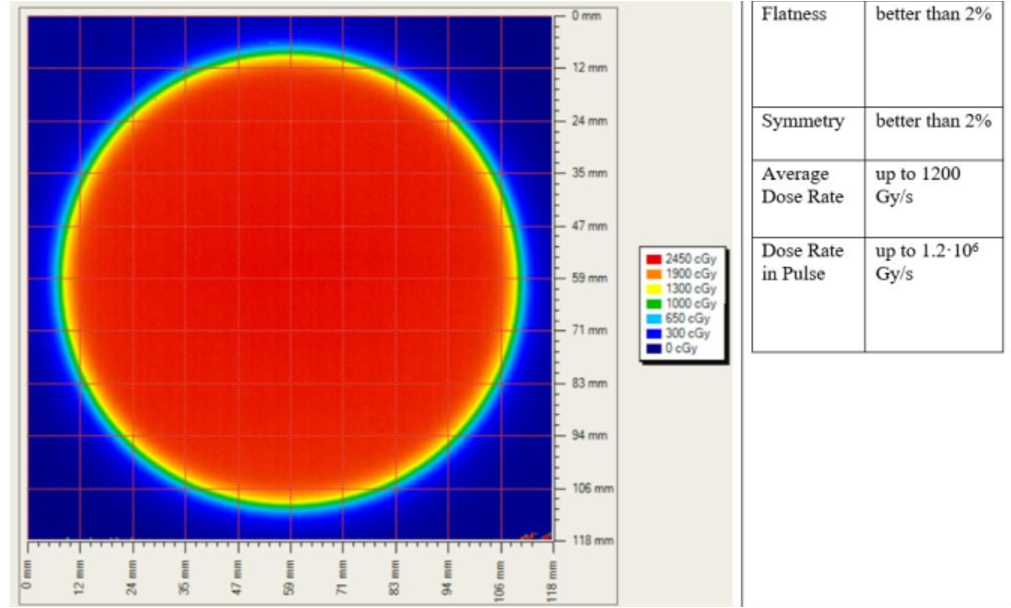
\includegraphics[width=.49\linewidth]{figures/test_beam/dose_profile_10cm.pdf}
         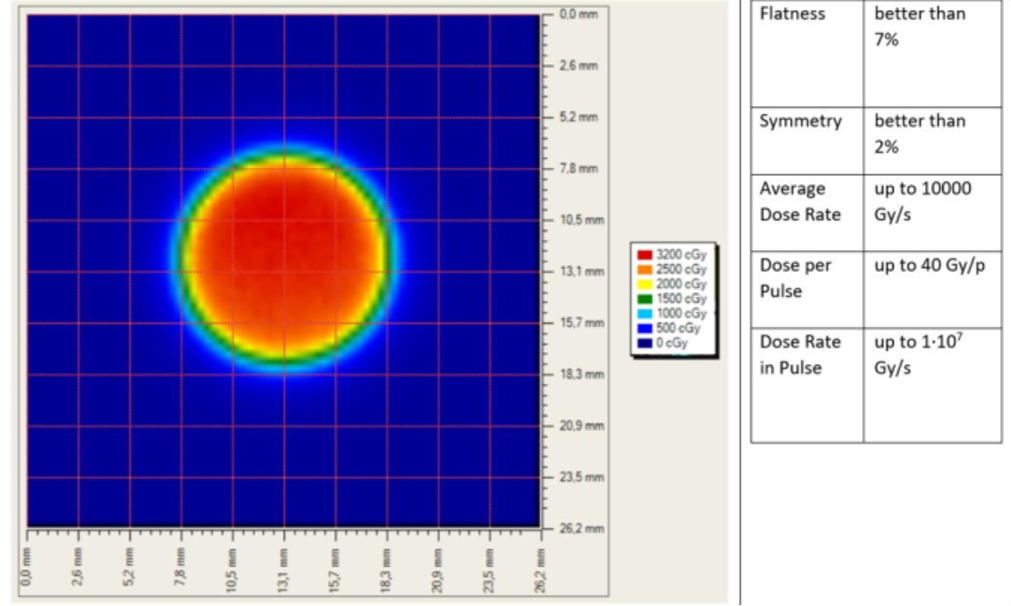
\includegraphics[width=.49\linewidth]{figures/test_beam/dose_profile_1cm.pdf}
         \caption{Two example of x-y isodose curves for two different triodes, \SI{10}{cm} and \SI{1}{cm} respectively, reported by the producer in the manual with the specific of the accelerator (S.I.T. - Sordina IORT Technologies S.p.A.). With the smaller collimator the dose rate in pulse is comparatively higher.}
         \label{fig:dose_profile}
      \end{figure}  

   \subsection{Mechanical carriers}
      The tested detector consists in one chip, the Device Under Test (DUT), mounted on a board and connected to FPGA with same arrangement of figure \ref{fig:}.
      These boards have been positioned vertically in front of the triode on a table specifically built for the testbeam. The tree board have been enclosed in a box of alluminium with a window on the DUT and with the required holes at the side to enable the biasing via cables and the connection with the DAQ provided via ethernet cable.       
      A trigger signal coming from the control unity and syncronized with the pulses emitted from the beam has been also sent to the FPGA.
      This digital signal cannot be considered a real trigger, since the TJ-Monopix1 prototype has been designed to be triggerless, but its Time of Arrival (ToA) had allowed the reconstruction of the correct timing during the analysis.

      In order to shield the sensor from the whole particles emitted from the gun, two alluminium collimators have been fabricated: one has been positioned at the triode exit while the other in front of the DUT. The collimators are $t$=\SI{32}{mm} thick and have a diameter $d$ equal to \SI{1}{mm}: assuming a beam divergence bigger than $d/t$=1/32 = \SI{1.8}{\degree}, which is the case, the collimator at the triode output was supposed to work as a point source and to reduce the rate on the DUT of a factor at least 4 10${^-4}$. The second one, being near the DUT, was instead supposed to shield the sensor from the electrons which have passed the first one, except for a region of \SI{1}{mm\squared} configurable using \red{come si chiamano quei cacciavitini per settare la posizione? sliding trimmer?}.  
      \begin{figure}[h!]
         \centering
         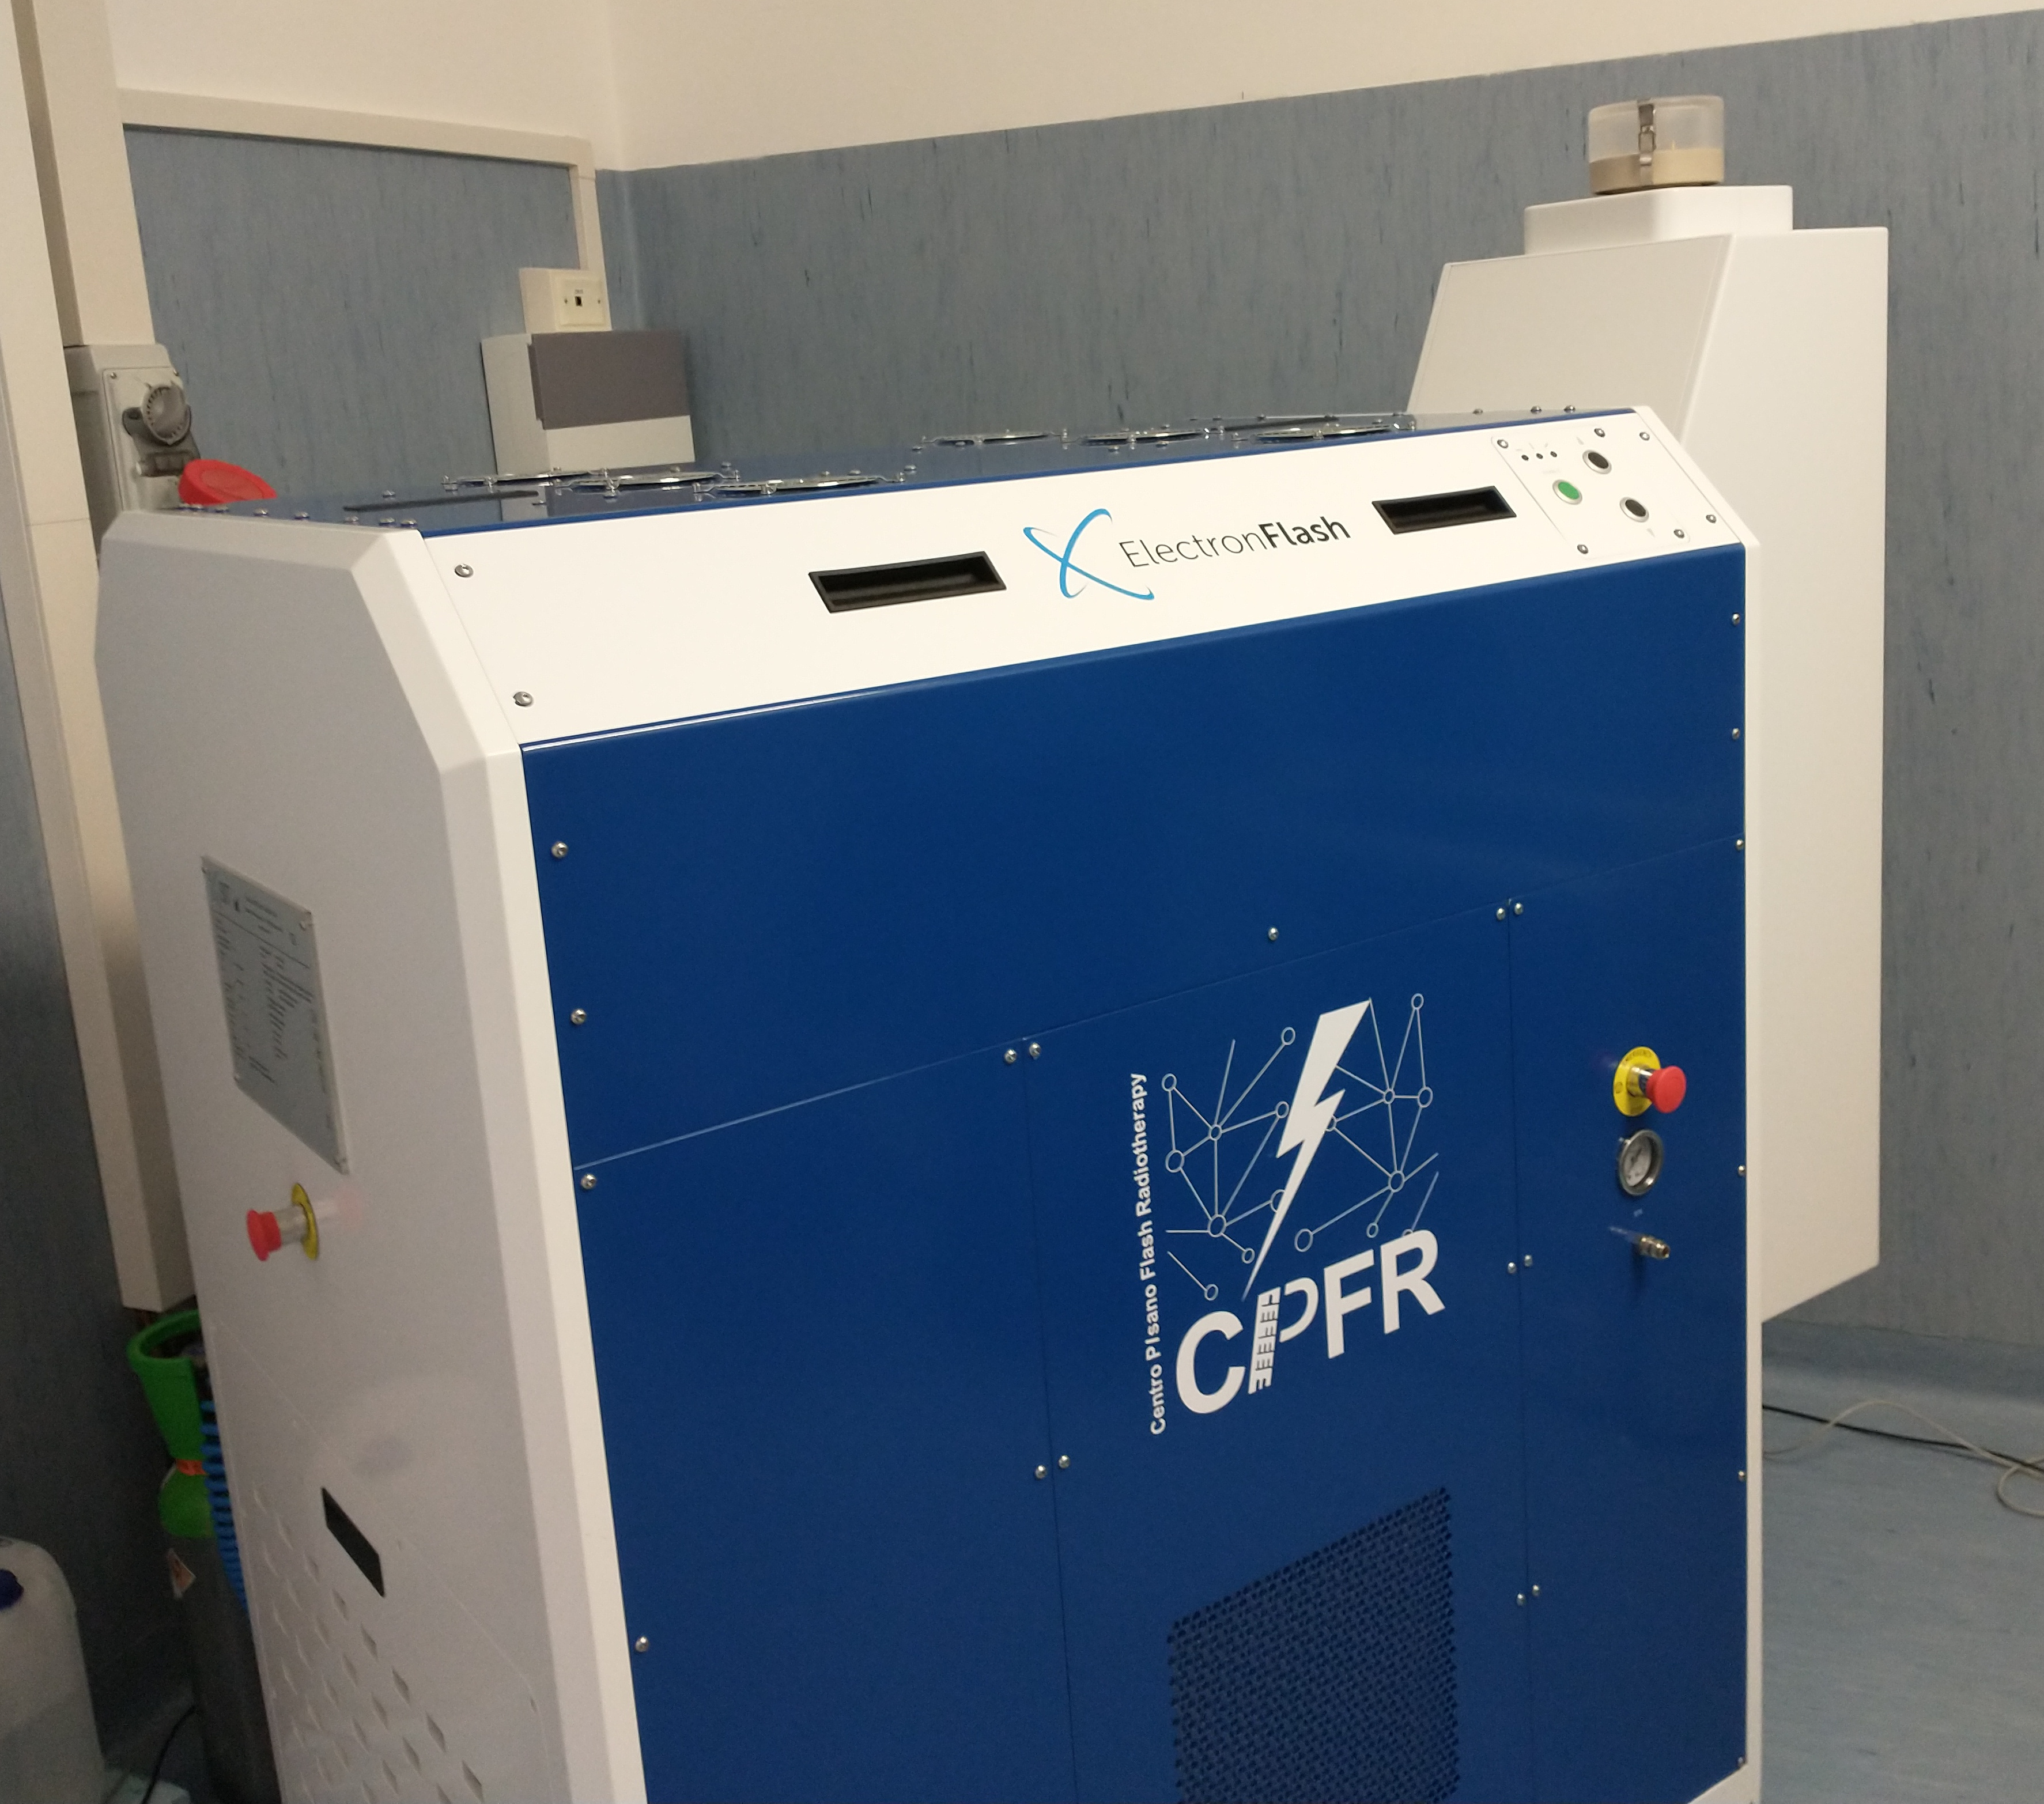
\includegraphics[width=.40\linewidth]{figures/test_beam/electron_flash.jpg}
         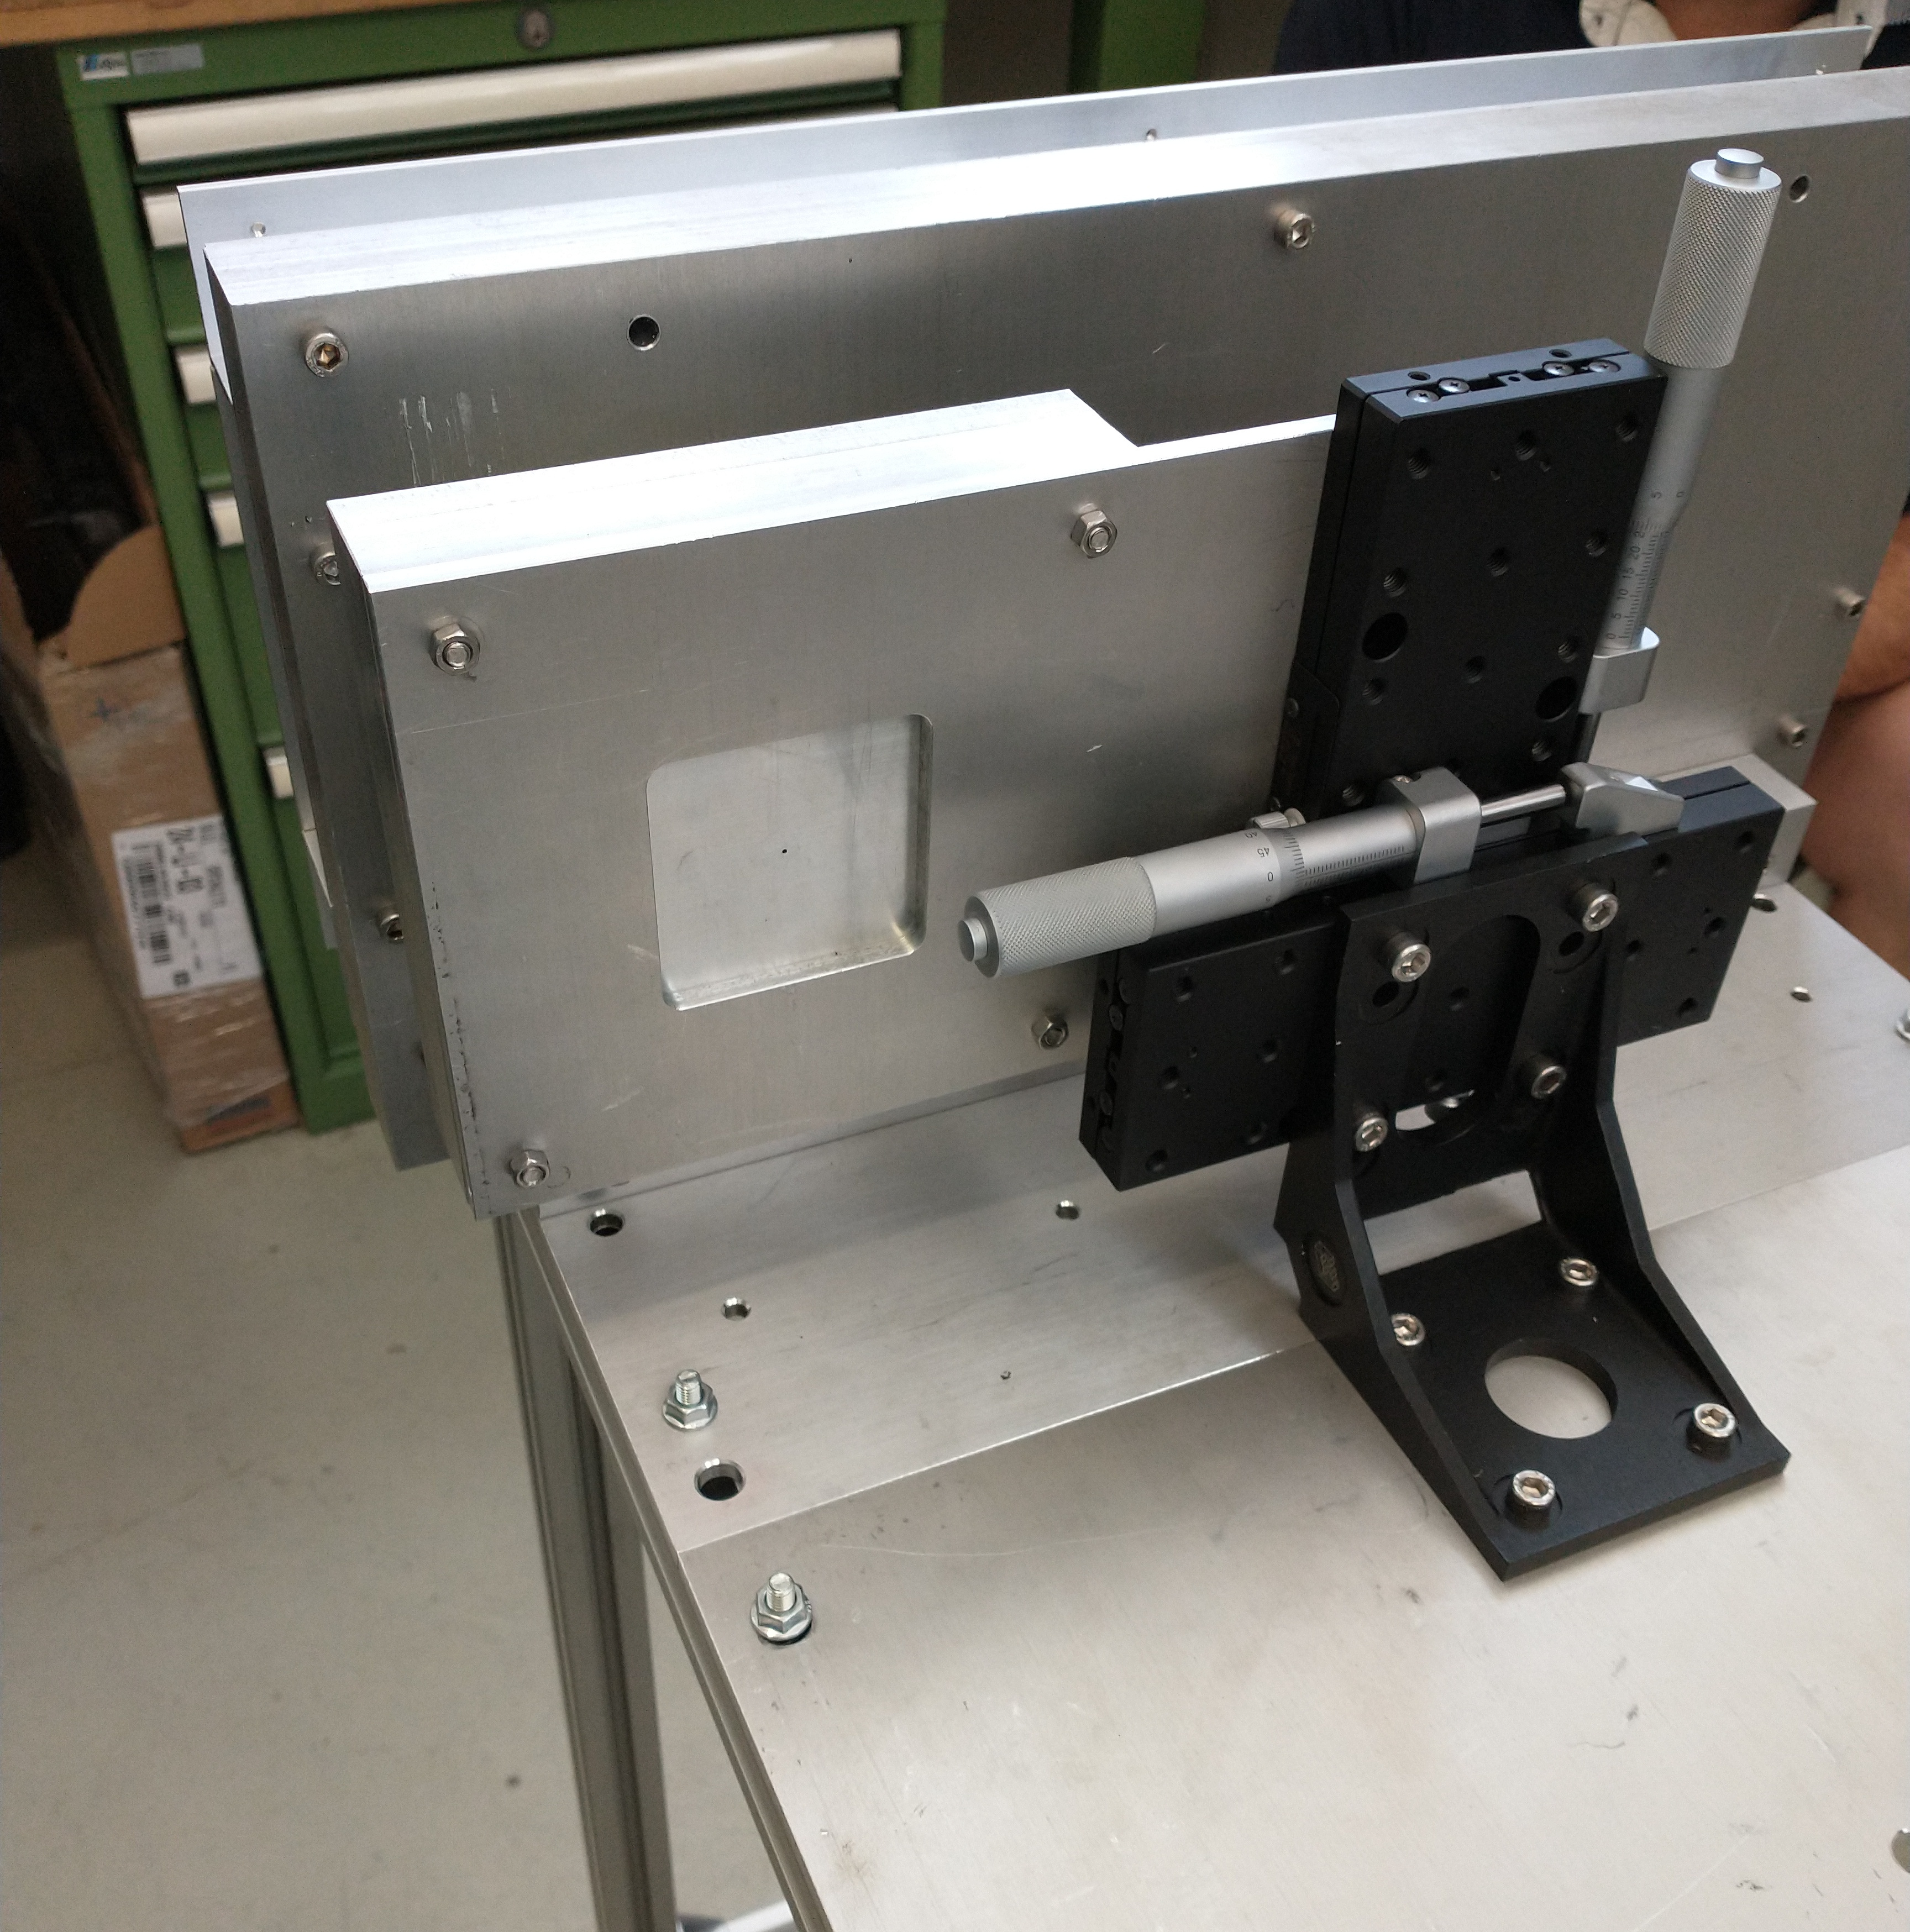
\includegraphics[width=.35\linewidth]{figures/test_beam/collimator_box.jpg}\\     
         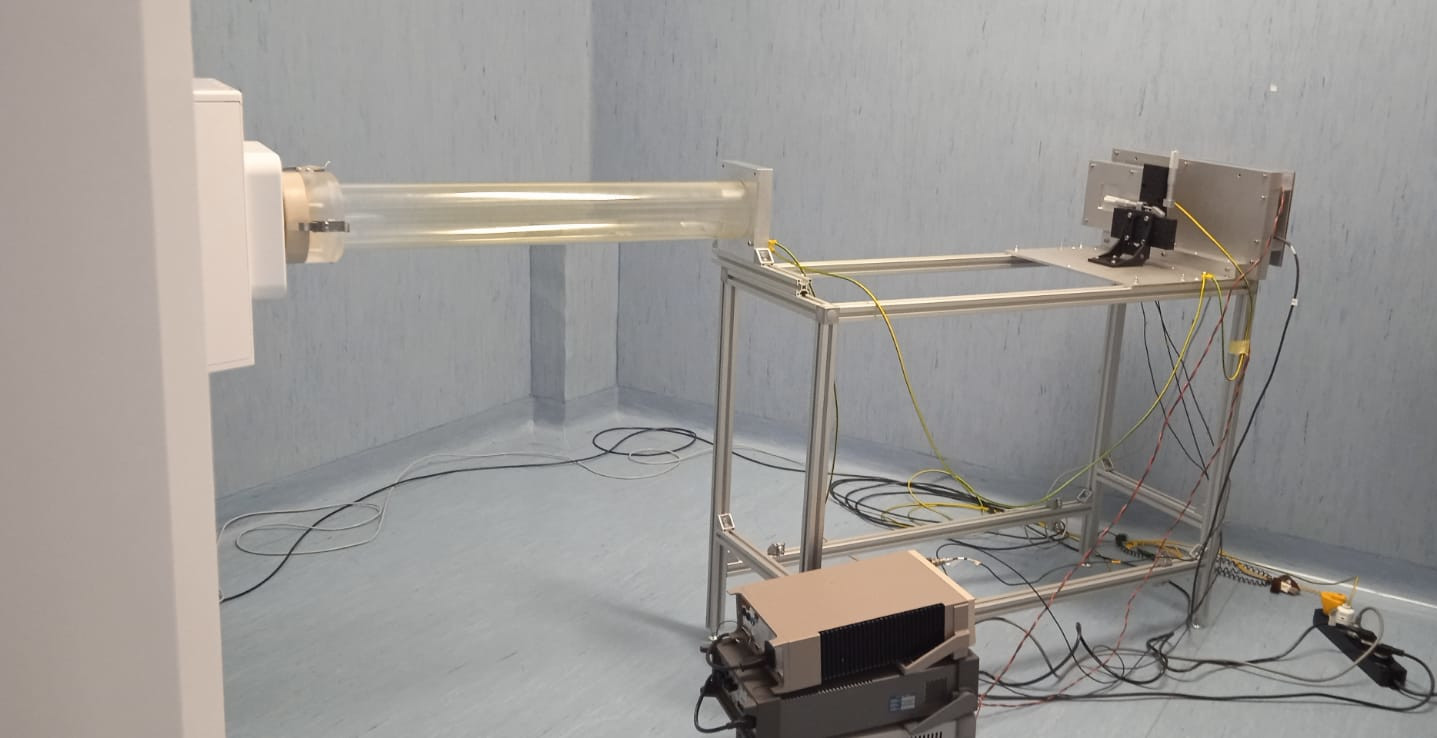
\includegraphics[width=.77\linewidth]{figures/test_beam/carrello.jpeg} 
         \label{fig:set_up}
         \caption{Experimental set up. (a) ElectronFlash accelerator: a
         rotating gantry allows the gun orientation from \SIrange{0}{90}{\degree} (horizontal /vertical). (b) Collimator and DUT box. (c) Whole structure mounted: we used the \SI{10}{cm} diameter and \SI{1.2}{m} long triode; the DUT which is in the box behind the two collimators is connected to the power supply units.}
      \end{figure}  

\section{Measurements}\label{sec:Santa_chiara_measurement}
   Because of the dead time of TJ-Monopix1 it is not possible resolving the bunch sub-structure and almost no one pixel can read more than a hit per bunch. I recall, indeed, that the dead time per pixel depends on the location on the readout priority chain and for each pixel $\lesssim$\SI{1}{\us} are needed; therefore, assuming a pulse duration of \SI{4}{\us}, only a few pixels at the top of the priority chain (placed at the upper left on the matrix) can fire a second time, as they can be read a first time before the end of the pulse and then can be hit again.

   Since resolving the single electron track is impossible, a way this sensor could be used in such context is reducing its efficiency and taking advantage of the analog pile up and of the linearity of the analog output (ToT), in order to see a signal produced not by the single particle but by more electrons. 
   Reducing the efficiency and the sensibility of the sensor is essential in order to decrease the high charge signal produced in the epitaxial layer and mitigating the saturation limit: the smaller the output signal produced by a particle and the higher the fluence the detector can cope with.
   There is an obious limit in this context that is the ToT rollover, indeed, the signal stop giving information when this value has been overridden and is no more bijective.
   With the standard configuration of the FE parameters and the epitaxial layer completely depleted, a MIP produces a charge at the limit of representation with a 6-bit ToT; to obtain smaller output signals one can operate on the reduction of the gain.

   Recalling the results in section \ref{chap:characterization_section:bias}, I have shown that concerning the PMOS flavor B, reducing the bias from -\SI{6}{V} to \SI{0}{V} brings a reduction of efficiency down to \SI{40}{\%}, and a reduction in the gain of a factor $\sim$1/3, while the reduction of the gain of the preamplifier allows a reduction of \red{circa 10, ma da controllare}.
   
   In order to taking advantage of the analog pile up and integrating the charge, for semplicity assume of two electrons, the second one must hit the pixel before the ToT goes under the threshold. The general condition is then $\overline{\Delta T}<\overline{ToT}$, but if a high P$_\mu$($n\geqslant$1) is required, a lower $\overline{\Delta T}$ may be desired:
   \begin{equation}
      P(n\geqslant1) = \sum\limits_{n=1}^n \frac{e^{-\mu\;\mu^n}}{n!} = 1\;-\;P(0) = 1\;-\;e^{-\mu}
   \end{equation}
   \begin{equation}
      \mu = \frac{\overline{ToT}}{\overline{\Delta T}}
   \end{equation}
   If a P$_\mu$($n\geqslant$1) = 99\% then the $\overline{\Delta T}$ must be $\sim$0.22 $\overline{ToT}$. The ToT is in range [0,64] but since the rollover must be avoided, the $\overline{ToT}$ must be lower than 32, and then the minimum rate on the pixel must be \SI{1.25}{\MHz}. \\

   During the testbeam many runs have been performed, spanning the energy, the dose per pulse and the four possible configurations with/without the collimators. 
   We have collected data with the PMOS flavor A in the standard configuration: with the PWELL and PSUB biased at -\SI{6}{V} and set the standard default FE parameters reported in table \ref{tab:FE_default}.
   During all the data acquisitions we have selected on the control unit of the accelerator pulses with t$_p$ of \SI{4}{\um} and with the smallest PRF settable, which is \SI{1}{Hz}, in order to start in the most conservative working point exluding the digital pile up of events from different bunch.with In this conditions, even if the whole matrix turns on, the total readout time corresponds to 25000$\times$\SI{1}{\us}=\SI{25}{ms} is still lower than the time between two consecutive pulses.
   In figure \ref{fig:hits_FLASH} is shown the mean number of hits read during one accelerator pulse in different setup condition.
   \begin{figure}
      \centering
      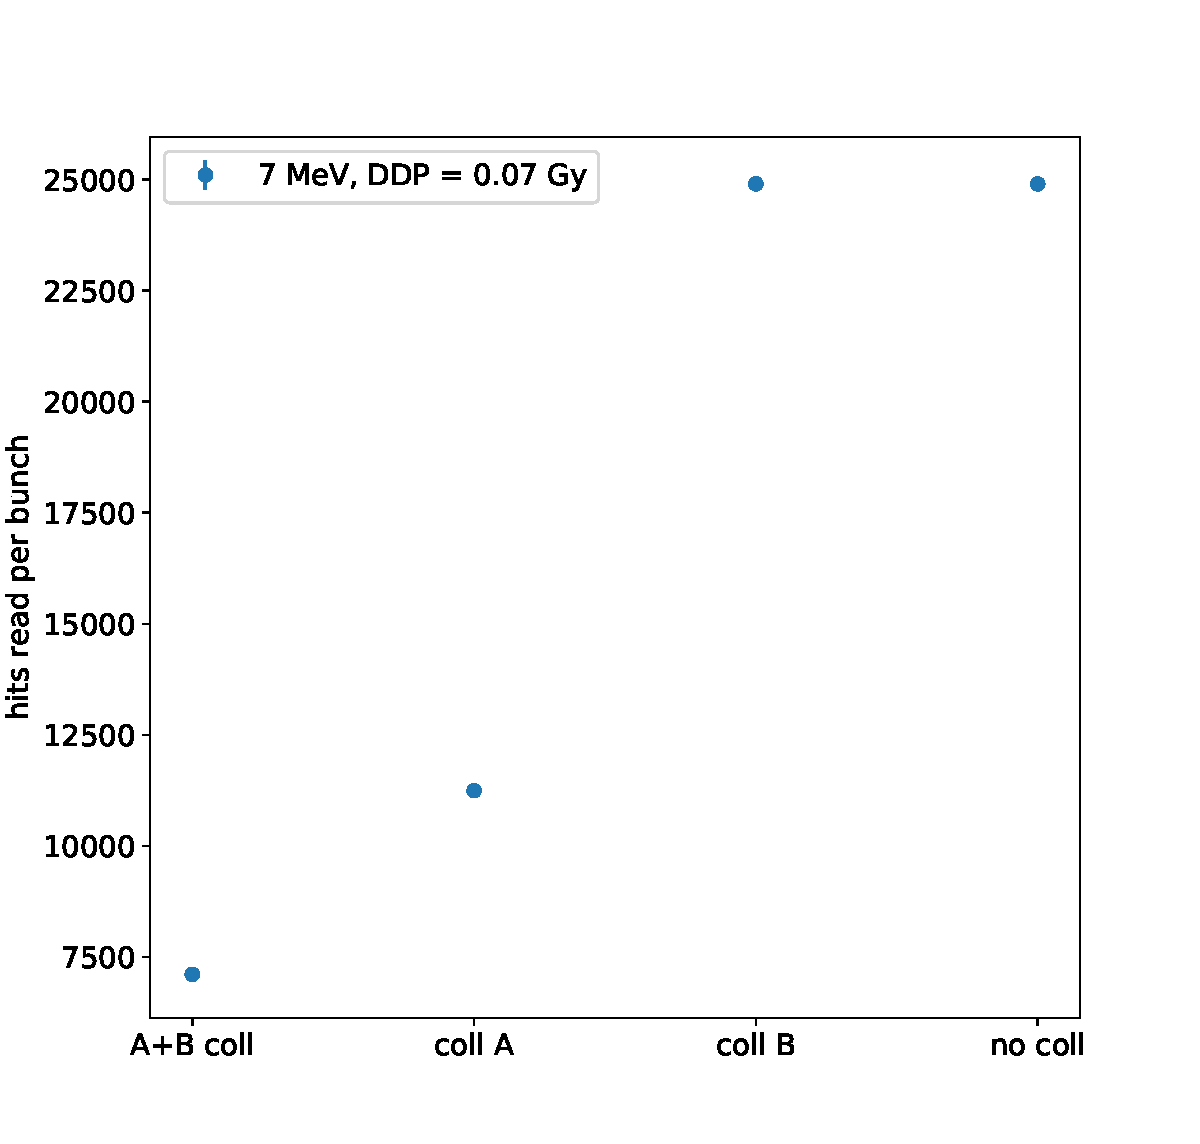
\includegraphics[width=.49\linewidth]{figures/test_beam/hits.pdf}
      \caption{Mean number of hits read per bunch at DDP=\SI{0.07}{Gy}, with all the possible setup condition: with both the collimator, with only the collimator far from the chip (A), with only the collimator near the chip (B), and without any collimator.}
      \label{fig:hits_FLASH}
   \end{figure}

   The readout starts with the trailing edge of the first pulse going down the threshold: about \SI{50}{clk}=\SI{1.25}{\us} after this moment the FREEZE signal is sent to the whole matrix, and the trasmittion of the data to the EoC begins.
   The hits read during the FREEZE signal are the ones whose TE occurred before the start of the FREEZE and which have the TOKEN signal high; the ones, instead, whose TE occur during the FREEZE are stored in the pixel memory until the end of the FREEZE. At this point a second readout starts and a second FREEZE is sent to the matrix.  
   An example of the two sub-pulses corresponding to an electron bunch is shown in figure \ref{fig:with_collimator}: in the acquisition we injected 5 pulses with both the collimators mounted on the table. 
   Looking at the spectrum we can see that the second sub-pulse has a populated tail on the right; this is due to the fact that the hits which arrive before the start of the first FREEZE but have a long ToT that falls during the FREEZE, are read at the second sub-pulse. 
   
   The 2D histograms in figure \ref{fig:with_collimator}, reveal an important charateristics of our setup: in fact, being uniform and not showing disomogenities, it follows that the collimators do not shield all the particles.
   We supposed that this was due to a Bremsstrahlung photon background higher than expected but a full verification of that and the analysis of the data is still going on. 
   In figure \ref{fig:hit_map_full_matrix}, instead, the histograms with a higher DDP value is shown; in the example the matrix turns on completely, but again this happens in two different consecutive read chain. 
   \begin{figure}
      \centering
      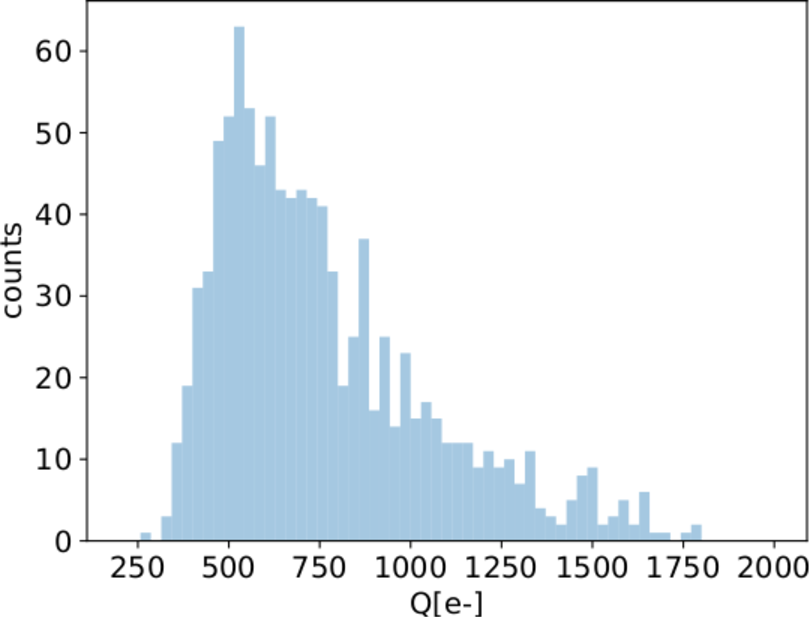
\includegraphics[width=.49\linewidth]{figures/test_beam/Q1_17_11.pdf}
      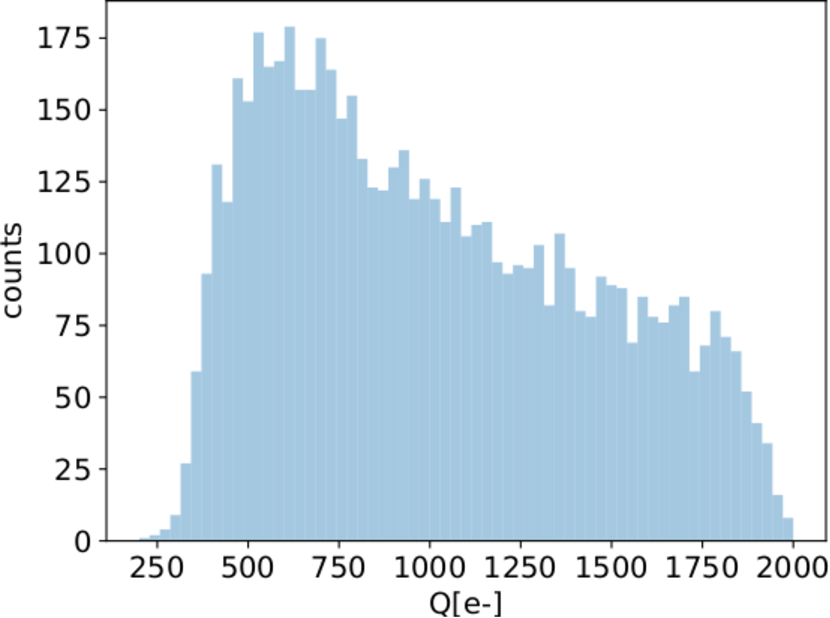
\includegraphics[width=.49\linewidth]{figures/test_beam/Q2_17_11.pdf}\\   
      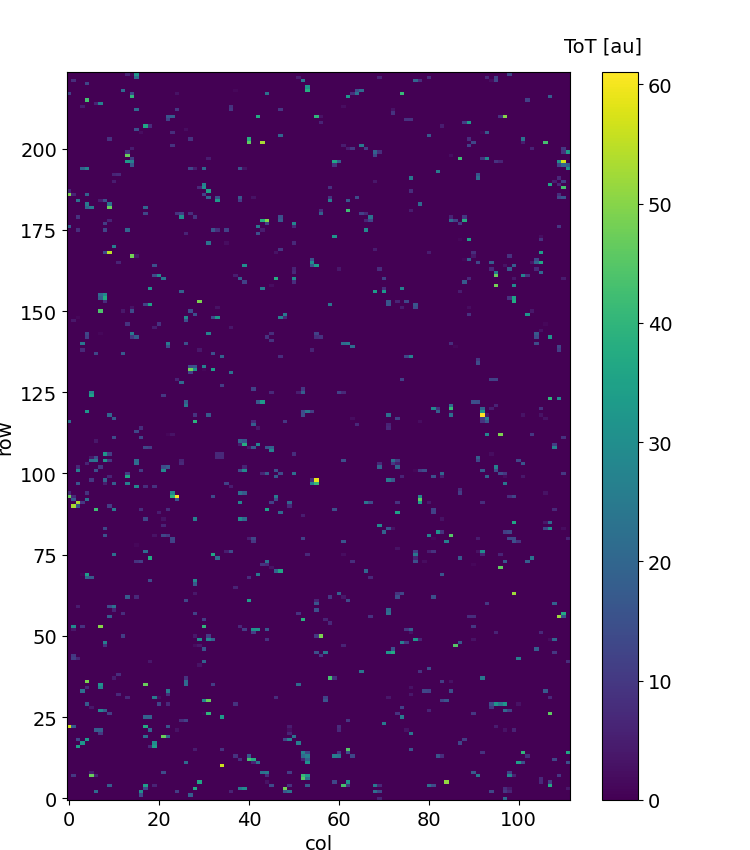
\includegraphics[width=.49\linewidth]{figures/test_beam/tot_mapq1_17-11.png}
      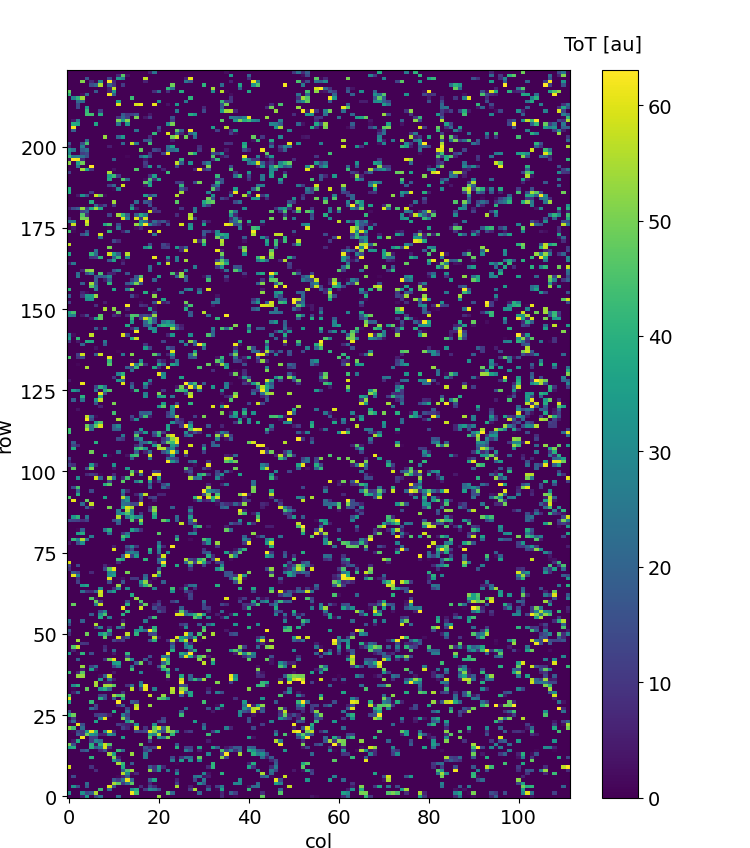
\includegraphics[width=.49\linewidth]{figures/test_beam/tot_mapq2_17-11.png} 
      \caption{Acquisition with both the collimators: 5 pulses at DDP=\SI{0.07}{Gy}. (a) Spectrum of the charge released in the sensor: to apply the conversion I used the information found in the previous chapter. (b) 2D histogram of the ToT of the hits arrived in the sub-pulses. }
      \label{fig:with_collimator}
   \end{figure}
   \begin{figure}
      \centering
      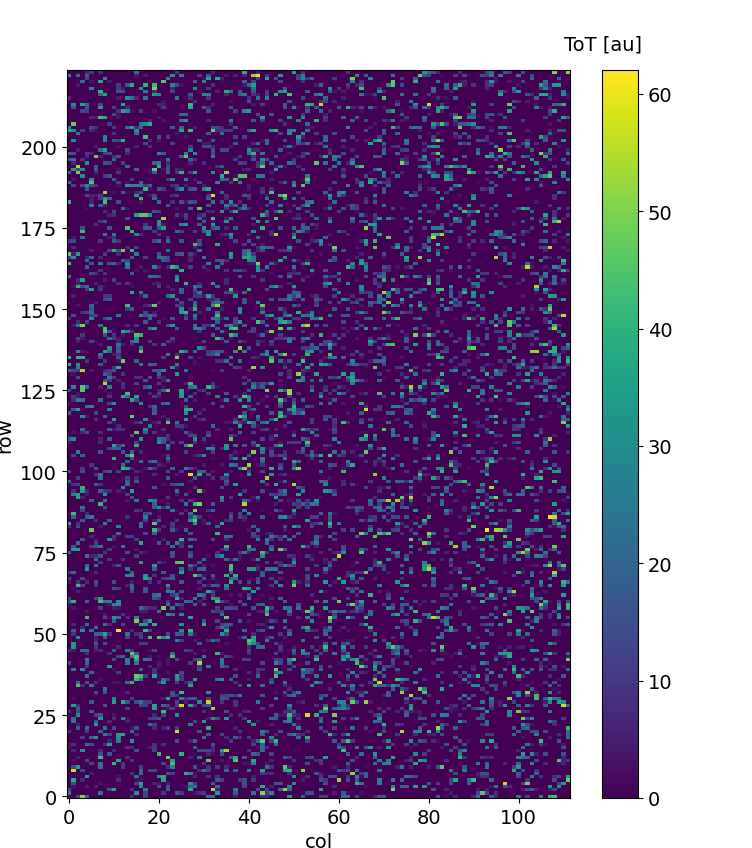
\includegraphics[width=.49\linewidth]{figures/test_beam/tot_mapq1_15-57.png}
      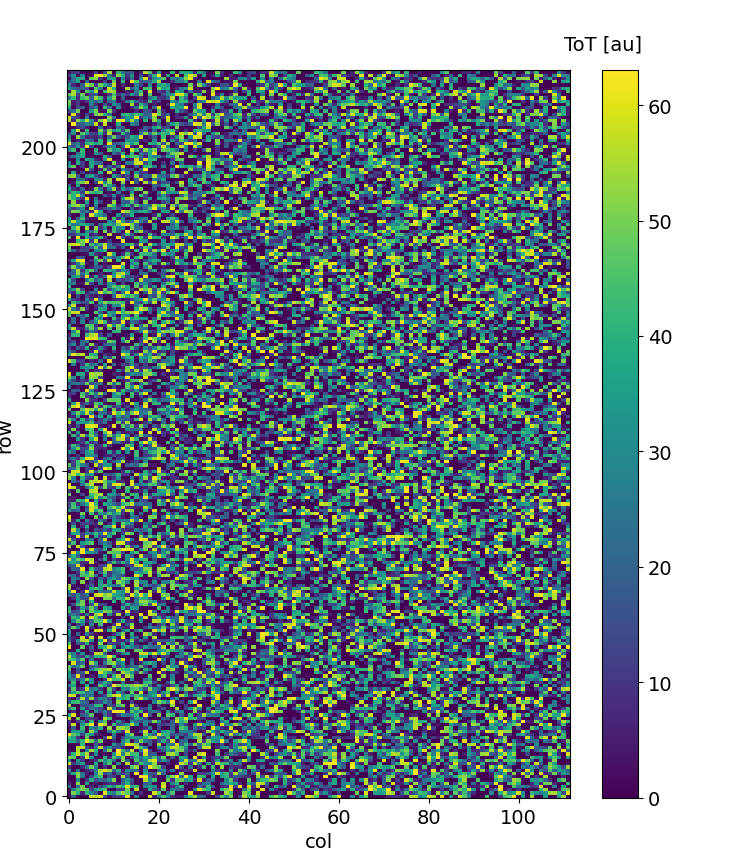
\includegraphics[width=.49\linewidth]{figures/test_beam/tot_mapq2_15-57.png}  
      \caption{Acquisition with both the collimators: 5 pulses at DDP=\SI{0.6}{Gy}. 2D histogram of the ToT of the hits arrived in the sub-pulses. Compared with the previous maps, since the DDP is much higher, more pixels turn on.}
      \label{fig:hit_map_full_matrix}
   \end{figure}



   When we have put aside the collimators, instead, the fluence increase a lot and the two-pulses substructure no more appears (fig. \ref{fig:without_collimator}), but, beacuse of the high attivity of the matrix, after each readout new hits with a fixed ToT were induced due to crosstalk.  
   This problem had already been observed on other prototypes of TJ-Monopix1, and thanks to a simulation it has been observed that the main source of crosstalk is the voltage drop of the pre-amplifier ground as a result of the accumulated current that is drawn from the discriminator.   
   \begin{figure}
      \centering
      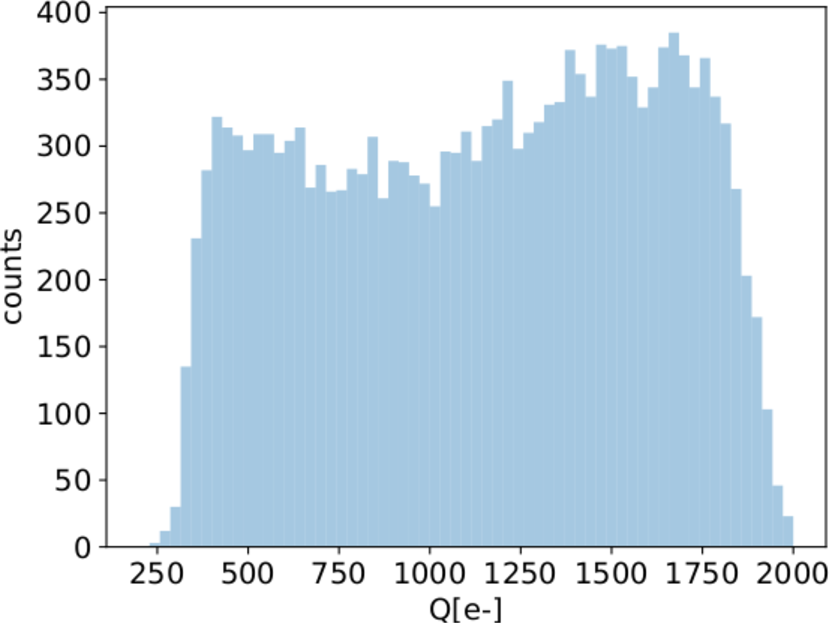
\includegraphics[width=.49\linewidth]{figures/test_beam/Qe_17_32.pdf}
      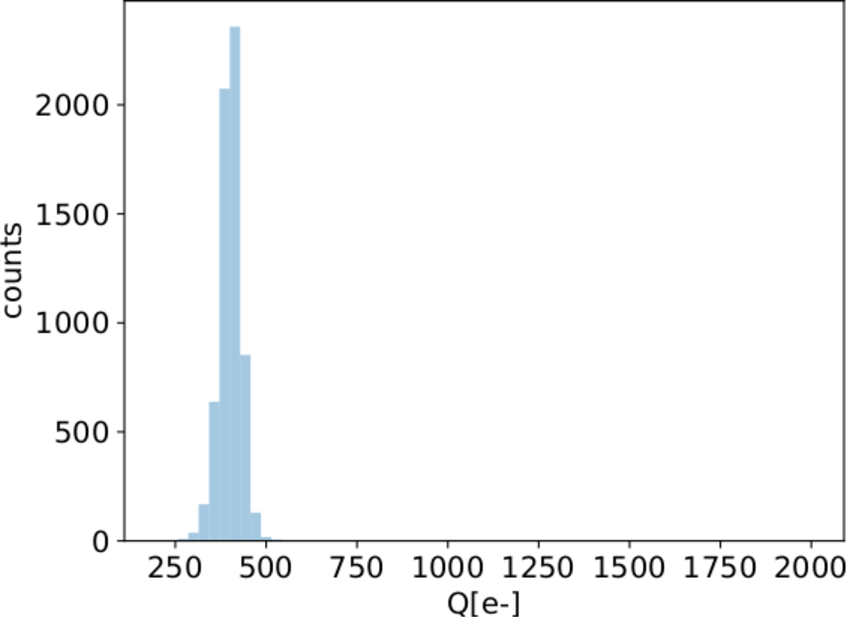
\includegraphics[width=.49\linewidth]{figures/test_beam/noise_Qe_17_32.pdf}
      \caption{Acquisition without any collimator: 5 pulses at DDP=\SI{0.04}{Gy}.}
      \label{fig:without_collimator}
   \end{figure}





   %\red{At PRF smaller than 100 Hz, all the dosimeters analyzed have
   %a shorter signal collection time with respect to the repetition
   %time of the pualses (maggiore uguale 10 ms), and, consequently, the %saturation
   %is influenced only by the dose-per-pulse (duration of the pulse is
   %around 2.5 us)}
   